\documentclass{standalone}
\usepackage{tikz}
\usetikzlibrary{patterns, positioning}


\begin{document}
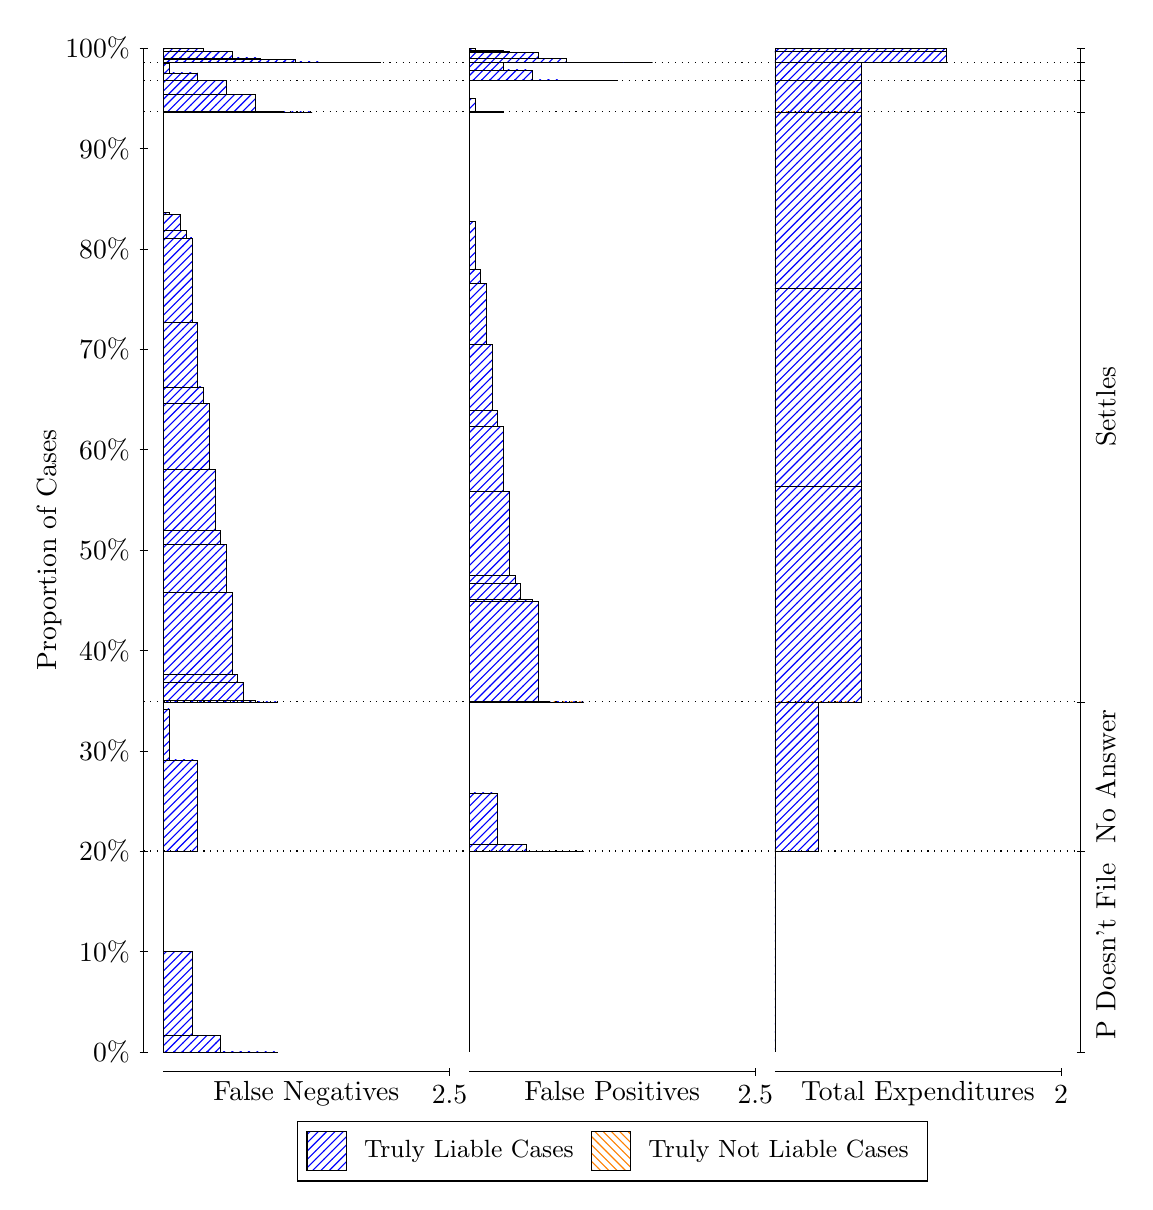
\begin{tikzpicture}
\draw[black, very thin] (1.5,1.75) -- (1.5,14.5);
\node[rotate=90, text=black, anchor=center] at (0.3, 8.125) {Proportion of Cases};
\draw[black, very thin] (1.45,1.75) -- (1.55,1.75);
\node[text=black, anchor=east] at (1.45, 1.75) {0\%};
\draw[black, very thin] (1.45,3.025) -- (1.55,3.025);
\node[text=black, anchor=east] at (1.45, 3.025) {10\%};
\draw[black, very thin] (1.45,4.3) -- (1.55,4.3);
\node[text=black, anchor=east] at (1.45, 4.3) {20\%};
\draw[black, very thin] (1.45,5.575) -- (1.55,5.575);
\node[text=black, anchor=east] at (1.45, 5.575) {30\%};
\draw[black, very thin] (1.45,6.85) -- (1.55,6.85);
\node[text=black, anchor=east] at (1.45, 6.85) {40\%};
\draw[black, very thin] (1.45,8.125) -- (1.55,8.125);
\node[text=black, anchor=east] at (1.45, 8.125) {50\%};
\draw[black, very thin] (1.45,9.4) -- (1.55,9.4);
\node[text=black, anchor=east] at (1.45, 9.4) {60\%};
\draw[black, very thin] (1.45,10.675) -- (1.55,10.675);
\node[text=black, anchor=east] at (1.45, 10.675) {70\%};
\draw[black, very thin] (1.45,11.95) -- (1.55,11.95);
\node[text=black, anchor=east] at (1.45, 11.95) {80\%};
\draw[black, very thin] (1.45,13.225) -- (1.55,13.225);
\node[text=black, anchor=east] at (1.45, 13.225) {90\%};
\draw[black, very thin] (1.45,14.5) -- (1.55,14.5);
\node[text=black, anchor=east] at (1.45, 14.5) {100\%};

\draw[black, very thin] (13.4,1.75) -- (13.4,14.5);
\draw[black, very thin] (13.35,1.75) -- (13.45,1.75);
\node[anchor=west] at (13.35, 1.75) {};
\draw[black, very thin] (13.35,4.3019) -- (13.45,4.3019);
\node[anchor=west] at (13.35, 4.3019) {};
\draw[black, very thin] (13.35,6.1967) -- (13.45,6.1967);
\node[anchor=west] at (13.35, 6.1967) {};
\draw[black, very thin] (13.35,13.69) -- (13.45,13.69);
\node[anchor=west] at (13.35, 13.69) {};
\draw[black, very thin] (13.35,14.087) -- (13.45,14.087);
\node[anchor=west] at (13.35, 14.087) {};
\draw[black, very thin] (13.35,14.32) -- (13.45,14.32);
\node[anchor=west] at (13.35, 14.32) {};
\draw[black, very thin] (13.35,14.5) -- (13.45,14.5);
\node[anchor=west] at (13.35, 14.5) {};

\draw[black, very thin, pattern color=blue, pattern=north east lines] (1.75,1.75) rectangle (3.2033,1.75);
\draw[black, very thin, pattern color=blue, pattern=north east lines] (1.75,1.75) rectangle (2.84,1.7521);
\draw[black, very thin, pattern color=blue, pattern=north east lines] (1.75,1.7521) rectangle (2.4767,1.9561);
\draw[black, very thin, pattern color=blue, pattern=north east lines] (1.75,1.9561) rectangle (2.1133,3.0289);
\draw[black, very thin, pattern color=orange, pattern=north west lines] (1.75,3.0289) rectangle (1.75,3.0289);
\draw[black, very thin, pattern color=blue, pattern=north east lines] (1.75,3.0289) rectangle (1.75,4.3019);
\draw[black, very thin, pattern color=blue, pattern=north east lines] (1.75,4.3019) rectangle (2.186,5.4591);
\draw[black, very thin, pattern color=blue, pattern=north east lines] (1.75,5.4591) rectangle (1.8227,6.1077);
\draw[black, very thin, pattern color=orange, pattern=north west lines] (1.75,6.1077) rectangle (1.75,6.1077);
\draw[black, very thin, pattern color=blue, pattern=north east lines] (1.75,6.1077) rectangle (1.75,6.1967);
\draw[black, very thin, pattern color=blue, pattern=north east lines] (1.75,6.1967) rectangle (3.2033,6.1967);
\draw[black, very thin, pattern color=blue, pattern=north east lines] (1.75,6.1967) rectangle (3.058,6.1969);
\draw[black, very thin, pattern color=blue, pattern=north east lines] (1.75,6.1969) rectangle (2.9127,6.2178);
\draw[black, very thin, pattern color=blue, pattern=north east lines] (1.75,6.2178) rectangle (2.84,6.2183);
\draw[black, very thin, pattern color=blue, pattern=north east lines] (1.75,6.2183) rectangle (2.7673,6.4443);
\draw[black, very thin, pattern color=blue, pattern=north east lines] (1.75,6.4443) rectangle (2.6947,6.5448);
\draw[black, very thin, pattern color=blue, pattern=north east lines] (1.75,6.5448) rectangle (2.622,7.5906);
\draw[black, very thin, pattern color=blue, pattern=north east lines] (1.75,7.5906) rectangle (2.5493,8.1983);
\draw[black, very thin, pattern color=blue, pattern=north east lines] (1.75,8.1983) rectangle (2.4767,8.3735);
\draw[black, very thin, pattern color=blue, pattern=north east lines] (1.75,8.3735) rectangle (2.404,9.1468);
\draw[black, very thin, pattern color=blue, pattern=north east lines] (1.75,9.1468) rectangle (2.3313,9.9866);
\draw[black, very thin, pattern color=blue, pattern=north east lines] (1.75,9.9866) rectangle (2.2587,10.196);
\draw[black, very thin, pattern color=blue, pattern=north east lines] (1.75,10.196) rectangle (2.186,11.016);
\draw[black, very thin, pattern color=blue, pattern=north east lines] (1.75,11.016) rectangle (2.1133,12.088);
\draw[black, very thin, pattern color=blue, pattern=north east lines] (1.75,12.088) rectangle (2.0407,12.183);
\draw[black, very thin, pattern color=blue, pattern=north east lines] (1.75,12.183) rectangle (1.968,12.386);
\draw[black, very thin, pattern color=blue, pattern=north east lines] (1.75,12.386) rectangle (1.8953,12.388);
\draw[black, very thin, pattern color=blue, pattern=north east lines] (1.75,12.388) rectangle (1.8227,12.415);
\draw[black, very thin, pattern color=orange, pattern=north west lines] (1.75,12.415) rectangle (1.75,12.415);
\draw[black, very thin, pattern color=blue, pattern=north east lines] (1.75,12.415) rectangle (1.75,13.69);
\draw[black, very thin, pattern color=blue, pattern=north east lines] (1.75,13.69) rectangle (3.6393,13.69);
\draw[black, very thin, pattern color=blue, pattern=north east lines] (1.75,13.69) rectangle (3.276,13.695);
\draw[black, very thin, pattern color=blue, pattern=north east lines] (1.75,13.695) rectangle (2.9127,13.913);
\draw[black, very thin, pattern color=blue, pattern=north east lines] (1.75,13.913) rectangle (2.5493,14.085);
\draw[black, very thin, pattern color=blue, pattern=north east lines] (1.75,14.085) rectangle (2.186,14.087);
\draw[black, very thin, pattern color=orange, pattern=north west lines] (1.75,14.087) rectangle (1.75,14.087);
\draw[black, very thin, pattern color=blue, pattern=north east lines] (1.75,14.087) rectangle (2.186,14.185);
\draw[black, very thin, pattern color=blue, pattern=north east lines] (1.75,14.185) rectangle (1.8227,14.312);
\draw[black, very thin, pattern color=orange, pattern=north west lines] (1.75,14.312) rectangle (1.75,14.312);
\draw[black, very thin, pattern color=blue, pattern=north east lines] (1.75,14.312) rectangle (1.75,14.32);
\draw[black, very thin, pattern color=blue, pattern=north east lines] (1.75,14.32) rectangle (4.5113,14.32);
\draw[black, very thin, pattern color=blue, pattern=north east lines] (1.75,14.32) rectangle (4.148,14.32);
\draw[black, very thin, pattern color=blue, pattern=north east lines] (1.75,14.32) rectangle (3.7847,14.324);
\draw[black, very thin, pattern color=blue, pattern=north east lines] (1.75,14.324) rectangle (3.712,14.324);
\draw[black, very thin, pattern color=blue, pattern=north east lines] (1.75,14.324) rectangle (3.4213,14.352);
\draw[black, very thin, pattern color=blue, pattern=north east lines] (1.75,14.352) rectangle (3.3487,14.352);
\draw[black, very thin, pattern color=blue, pattern=north east lines] (1.75,14.352) rectangle (3.058,14.36);
\draw[black, very thin, pattern color=blue, pattern=north east lines] (1.75,14.36) rectangle (2.9853,14.374);
\draw[black, very thin, pattern color=blue, pattern=north east lines] (1.75,14.374) rectangle (2.6947,14.374);
\draw[black, very thin, pattern color=blue, pattern=north east lines] (1.75,14.374) rectangle (2.622,14.456);
\draw[black, very thin, pattern color=blue, pattern=north east lines] (1.75,14.456) rectangle (2.3313,14.456);
\draw[black, very thin, pattern color=blue, pattern=north east lines] (1.75,14.456) rectangle (2.2587,14.498);
\draw[black, very thin, pattern color=blue, pattern=north east lines] (1.75,14.498) rectangle (1.8953,14.5);
\draw[black, very thin, pattern color=orange, pattern=north west lines] (1.75,14.5) rectangle (1.75,14.5);
\draw[black, very thin, pattern color=blue, pattern=north east lines] (1.75,14.5) rectangle (1.75,14.5);
\draw[black, very thin, pattern color=orange, pattern=north west lines] (5.6333,1.75) rectangle (5.6333,1.75);
\draw[black, very thin, pattern color=blue, pattern=north east lines] (5.6333,1.75) rectangle (5.6333,4.3019);
\draw[black, very thin, pattern color=orange, pattern=north west lines] (5.6333,4.3019) rectangle (7.0867,4.3019);
\draw[black, very thin, pattern color=blue, pattern=north east lines] (5.6333,4.3019) rectangle (7.0867,4.3019);
\draw[black, very thin, pattern color=blue, pattern=north east lines] (5.6333,4.3019) rectangle (6.7233,4.3021);
\draw[black, very thin, pattern color=blue, pattern=north east lines] (5.6333,4.3021) rectangle (6.36,4.3909);
\draw[black, very thin, pattern color=blue, pattern=north east lines] (5.6333,4.3909) rectangle (5.9967,5.0395);
\draw[black, very thin, pattern color=blue, pattern=north east lines] (5.6333,5.0395) rectangle (5.6333,6.1967);
\draw[black, very thin, pattern color=orange, pattern=north west lines] (5.6333,6.1967) rectangle (7.0867,6.1967);
\draw[black, very thin, pattern color=blue, pattern=north east lines] (5.6333,6.1967) rectangle (7.0867,6.1967);
\draw[black, very thin, pattern color=orange, pattern=north west lines] (5.6333,6.1967) rectangle (6.9413,6.1967);
\draw[black, very thin, pattern color=blue, pattern=north east lines] (5.6333,6.1967) rectangle (6.9413,6.1967);
\draw[black, very thin, pattern color=orange, pattern=north west lines] (5.6333,6.1967) rectangle (6.796,6.1967);
\draw[black, very thin, pattern color=blue, pattern=north east lines] (5.6333,6.1967) rectangle (6.796,6.1967);
\draw[black, very thin, pattern color=blue, pattern=north east lines] (5.6333,6.1967) rectangle (6.7233,6.1967);
\draw[black, very thin, pattern color=orange, pattern=north west lines] (5.6333,6.1967) rectangle (6.6507,6.1967);
\draw[black, very thin, pattern color=blue, pattern=north east lines] (5.6333,6.1967) rectangle (6.6507,6.1988);
\draw[black, very thin, pattern color=blue, pattern=north east lines] (5.6333,6.1988) rectangle (6.578,6.1989);
\draw[black, very thin, pattern color=orange, pattern=north west lines] (5.6333,6.1989) rectangle (6.5053,6.1989);
\draw[black, very thin, pattern color=blue, pattern=north east lines] (5.6333,6.1989) rectangle (6.5053,7.4719);
\draw[black, very thin, pattern color=blue, pattern=north east lines] (5.6333,7.4719) rectangle (6.4327,7.4989);
\draw[black, very thin, pattern color=blue, pattern=north east lines] (5.6333,7.4989) rectangle (6.36,7.5009);
\draw[black, very thin, pattern color=blue, pattern=north east lines] (5.6333,7.5009) rectangle (6.2873,7.7036);
\draw[black, very thin, pattern color=blue, pattern=north east lines] (5.6333,7.7036) rectangle (6.2147,7.7992);
\draw[black, very thin, pattern color=blue, pattern=north east lines] (5.6333,7.7992) rectangle (6.142,8.8712);
\draw[black, very thin, pattern color=blue, pattern=north east lines] (5.6333,8.8712) rectangle (6.0693,9.6915);
\draw[black, very thin, pattern color=blue, pattern=north east lines] (5.6333,9.6915) rectangle (5.9967,9.9004);
\draw[black, very thin, pattern color=blue, pattern=north east lines] (5.6333,9.9004) rectangle (5.924,10.74);
\draw[black, very thin, pattern color=blue, pattern=north east lines] (5.6333,10.74) rectangle (5.8513,11.513);
\draw[black, very thin, pattern color=blue, pattern=north east lines] (5.6333,11.513) rectangle (5.7787,11.689);
\draw[black, very thin, pattern color=blue, pattern=north east lines] (5.6333,11.689) rectangle (5.706,12.296);
\draw[black, very thin, pattern color=blue, pattern=north east lines] (5.6333,12.296) rectangle (5.6333,13.69);
\draw[black, very thin, pattern color=orange, pattern=north west lines] (5.6333,13.69) rectangle (6.0693,13.69);
\draw[black, very thin, pattern color=blue, pattern=north east lines] (5.6333,13.69) rectangle (6.0693,13.692);
\draw[black, very thin, pattern color=blue, pattern=north east lines] (5.6333,13.692) rectangle (5.706,13.865);
\draw[black, very thin, pattern color=blue, pattern=north east lines] (5.6333,13.865) rectangle (5.6333,14.087);
\draw[black, very thin, pattern color=orange, pattern=north west lines] (5.6333,14.087) rectangle (7.5227,14.087);
\draw[black, very thin, pattern color=blue, pattern=north east lines] (5.6333,14.087) rectangle (7.5227,14.087);
\draw[black, very thin, pattern color=blue, pattern=north east lines] (5.6333,14.087) rectangle (7.1593,14.087);
\draw[black, very thin, pattern color=blue, pattern=north east lines] (5.6333,14.087) rectangle (6.796,14.095);
\draw[black, very thin, pattern color=blue, pattern=north east lines] (5.6333,14.095) rectangle (6.4327,14.222);
\draw[black, very thin, pattern color=blue, pattern=north east lines] (5.6333,14.222) rectangle (6.0693,14.32);
\draw[black, very thin, pattern color=orange, pattern=north west lines] (5.6333,14.32) rectangle (7.9587,14.32);
\draw[black, very thin, pattern color=blue, pattern=north east lines] (5.6333,14.32) rectangle (7.9587,14.32);
\draw[black, very thin, pattern color=orange, pattern=north west lines] (5.6333,14.32) rectangle (7.5953,14.32);
\draw[black, very thin, pattern color=blue, pattern=north east lines] (5.6333,14.32) rectangle (7.5953,14.32);
\draw[black, very thin, pattern color=orange, pattern=north west lines] (5.6333,14.32) rectangle (7.232,14.32);
\draw[black, very thin, pattern color=blue, pattern=north east lines] (5.6333,14.32) rectangle (7.232,14.322);
\draw[black, very thin, pattern color=blue, pattern=north east lines] (5.6333,14.322) rectangle (6.8687,14.364);
\draw[black, very thin, pattern color=orange, pattern=north west lines] (5.6333,14.364) rectangle (6.8687,14.364);
\draw[black, very thin, pattern color=blue, pattern=north east lines] (5.6333,14.364) rectangle (6.8687,14.364);
\draw[black, very thin, pattern color=orange, pattern=north west lines] (5.6333,14.364) rectangle (6.796,14.364);
\draw[black, very thin, pattern color=blue, pattern=north east lines] (5.6333,14.364) rectangle (6.796,14.364);
\draw[black, very thin, pattern color=blue, pattern=north east lines] (5.6333,14.364) rectangle (6.5053,14.445);
\draw[black, very thin, pattern color=blue, pattern=north east lines] (5.6333,14.445) rectangle (6.5053,14.446);
\draw[black, very thin, pattern color=orange, pattern=north west lines] (5.6333,14.446) rectangle (6.4327,14.446);
\draw[black, very thin, pattern color=blue, pattern=north east lines] (5.6333,14.446) rectangle (6.4327,14.446);
\draw[black, very thin, pattern color=blue, pattern=north east lines] (5.6333,14.446) rectangle (6.142,14.453);
\draw[black, very thin, pattern color=blue, pattern=north east lines] (5.6333,14.453) rectangle (6.142,14.46);
\draw[black, very thin, pattern color=blue, pattern=north east lines] (5.6333,14.46) rectangle (6.0693,14.468);
\draw[black, very thin, pattern color=orange, pattern=north west lines] (5.6333,14.468) rectangle (6.0693,14.468);
\draw[black, very thin, pattern color=blue, pattern=north east lines] (5.6333,14.468) rectangle (6.0693,14.468);
\draw[black, very thin, pattern color=blue, pattern=north east lines] (5.6333,14.468) rectangle (5.7787,14.468);
\draw[black, very thin, pattern color=blue, pattern=north east lines] (5.6333,14.468) rectangle (5.7787,14.468);
\draw[black, very thin, pattern color=blue, pattern=north east lines] (5.6333,14.468) rectangle (5.706,14.495);
\draw[black, very thin, pattern color=blue, pattern=north east lines] (5.6333,14.495) rectangle (5.706,14.496);
\draw[black, very thin, pattern color=blue, pattern=north east lines] (5.6333,14.496) rectangle (5.6333,14.5);
\draw[black, very thin, pattern color=orange, pattern=north west lines] (9.5167,1.75) rectangle (9.5167,1.75);
\draw[black, very thin, pattern color=blue, pattern=north east lines] (9.5167,1.75) rectangle (9.5167,4.3019);
\draw[black, very thin, pattern color=orange, pattern=north west lines] (9.5167,4.3019) rectangle (10.062,4.3019);
\draw[black, very thin, pattern color=blue, pattern=north east lines] (9.5167,4.3019) rectangle (10.062,6.1967);
\draw[black, very thin, pattern color=orange, pattern=north west lines] (9.5167,6.1967) rectangle (10.607,6.1967);
\draw[black, very thin, pattern color=blue, pattern=north east lines] (9.5167,6.1967) rectangle (10.607,8.9294);
\draw[black, very thin, pattern color=orange, pattern=north west lines] (9.5167,8.9294) rectangle (10.607,8.9294);
\draw[black, very thin, pattern color=blue, pattern=north east lines] (9.5167,8.9294) rectangle (10.607,11.45);
\draw[black, very thin, pattern color=orange, pattern=north west lines] (9.5167,11.45) rectangle (10.607,11.45);
\draw[black, very thin, pattern color=blue, pattern=north east lines] (9.5167,11.45) rectangle (10.607,13.69);
\draw[black, very thin, pattern color=orange, pattern=north west lines] (9.5167,13.69) rectangle (10.607,13.69);
\draw[black, very thin, pattern color=blue, pattern=north east lines] (9.5167,13.69) rectangle (10.607,14.087);
\draw[black, very thin, pattern color=orange, pattern=north west lines] (9.5167,14.087) rectangle (10.607,14.087);
\draw[black, very thin, pattern color=blue, pattern=north east lines] (9.5167,14.087) rectangle (10.607,14.32);
\draw[black, very thin, pattern color=orange, pattern=north west lines] (9.5167,14.32) rectangle (11.697,14.32);
\draw[black, very thin, pattern color=blue, pattern=north east lines] (9.5167,14.32) rectangle (11.697,14.453);
\draw[black, very thin, pattern color=orange, pattern=north west lines] (9.5167,14.453) rectangle (11.697,14.453);
\draw[black, very thin, pattern color=blue, pattern=north east lines] (9.5167,14.453) rectangle (11.697,14.5);
\draw[black, dotted] (1.5,4.3019) -- (13.4,4.3019);
\draw[black, dotted] (1.5,6.1967) -- (13.4,6.1967);
\draw[black, dotted] (1.5,13.69) -- (13.4,13.69);
\draw[black, dotted] (1.5,14.087) -- (13.4,14.087);
\draw[black, dotted] (1.5,14.32) -- (13.4,14.32);
\draw[black, very thin] (1.75,1.5) -- (5.3833,1.5);
\node[text=black, anchor=north] at (3.5667, 1.5) {False Negatives};
\draw[black, very thin] (5.3833,1.45) -- (5.3833,1.55);
\node[text=black, anchor=north] at (5.3833, 1.45) {2.5};

\draw[black, very thin] (5.6333,1.5) -- (9.2667,1.5);
\node[text=black, anchor=north] at (7.45, 1.5) {False Positives};
\draw[black, very thin] (9.2667,1.45) -- (9.2667,1.55);
\node[text=black, anchor=north] at (9.2667, 1.45) {2.5};

\draw[black, very thin] (9.5167,1.5) -- (13.15,1.5);
\node[text=black, anchor=north] at (11.333, 1.5) {Total Expenditures};
\draw[black, very thin] (13.15,1.45) -- (13.15,1.55);
\node[text=black, anchor=north] at (13.15, 1.45) {2};

\node[text=black, centered, rotate=90] at (13.72, 3.026) {P Doesn't File};
\node[text=black, centered, rotate=90] at (13.72, 5.2493) {No Answer};
\node[text=black, centered, rotate=90] at (13.72, 9.9435) {Settles};




\draw (7.449999999999999,1.5) node[draw=none] (baseCoordinate) {};
\begin{scope}[align=center]
        \matrix[scale=0.5, draw=black, below=0.5cm of baseCoordinate, nodes={draw}, column sep=0.1cm]{
            \node[rectangle, draw, minimum width=0.5cm, minimum height=0.5cm, pattern color=blue, pattern=north east lines] {}; &
            \node[draw=none, font=\small, text=black] (B) {Truly Liable Cases}; &
            \node[rectangle, draw, minimum width=0.5cm, minimum height=0.5cm, pattern color=orange, pattern=north west lines] {}; &
            \node[draw=none, font=\small, text=black] (B) {Truly Not Liable Cases}; \\
            };
\end{scope}

\end{tikzpicture}
\end{document}